%%%%%%%%%%%%%%%%%%%%%%%%%%%%%%%%%%%%%%%%%%%%%%%%%%%%%%%%%%%%
%%  This Beamer template was created by Cameron Bracken.
%%  Anyone can freely use or modify it for any purpose
%%  without attribution.
%%
%%  Last Modified: January 9, 2009
%%

\documentclass[xcolor=x11names,compress]{beamer}

%% General document %%%%%%%%%%%%%%%%%%%%%%%%%%%%%%%%%%
\usepackage[utf8]{inputenc}
\usepackage[ngerman]{babel}
\usepackage{graphicx}
\usepackage{color}
\usepackage{tikz}
\usepackage{tabularx}
\usepackage[skins]{tcolorbox}
\usepackage{caption}
\usepackage{csquotes}
\usepackage{multicol,listings}
\usepackage{multirow}
\usepackage[absolute,overlay]{textpos}
\usepackage{transparent}
\usepackage{enumitem}
%%%%%%%%%%%%%%%%%%%%%%%%%%%%%%%%%%%%%%%%%%%%%%%%%%%%%%

%% Beamer Layout %%%%%%%%%%%%%%%%%%%%%%%%%%%%%%%%%%
\useoutertheme[subsection=false,infolines]{miniframes}
\useinnertheme{default}
\usefonttheme{serif}
\usepackage{palatino}

\setbeamertemplate{footline}[frame number]
%\setbeamertemplate{caption}[numbered]
\setbeamercolor{page number in head/foot}{fg=black}

\setbeamerfont{title like}{shape=\scshape}
\setbeamerfont{frametitle}{shape=\scshape}
\setbeamerfont{caption}{size=\tiny}
\setbeamerfont{caption name}{size=\tiny}

\setbeamercolor*{lower separation line head}{bg=DeepSkyBlue4} 
\setbeamercolor*{normal text}{fg=black,bg=white} 
\setbeamercolor*{alerted text}{fg=red} 
\setbeamercolor*{example text}{fg=black} 
\setbeamercolor*{structure}{fg=black} 
 
\setbeamercolor*{palette tertiary}{fg=black,bg=black!10} 
\setbeamercolor*{palette quaternary}{fg=black,bg=black!10} 

% Set right item bullet points in itemize (due to enumitem package)
\setitemize{label=\usebeamerfont*{itemize item}%
  \usebeamercolor[fg]{itemize item}
  \usebeamertemplate{itemize item}}

\renewcommand{\(}{\begin{columns}}
\renewcommand{\)}{\end{columns}}
\newcommand{\<}[1]{\begin{column}{#1}}
\renewcommand{\>}{\end{column}}

\beamertemplatenavigationsymbolsempty
\setcounter{tocdepth}{1}

\tcbset{enhanced}

% Set color for lstlisting
\definecolor{grey}{RGB}{105,105,105}

%%%%%%%%%%%%%%%%%%%%%%%%%%%%%%%%%%%%%%%%%%%%%%%%%%


\begin{document}

\begin{frame}
  \begin{figure}
    \begin{minipage}[c]{0.6\textwidth} 
    \tiny{Humboldt University of Berlin\\Department of Computer Science\\Computer Engineering Group}
    \end{minipage}
    \hfill
    \begin{minipage}[c]{0.15\textwidth}
    \begin{figure}
      
\includegraphics[width=\textwidth]{figures/HU_Logo}
    \end{figure}
    \end{minipage}
  \end{figure}

\title{\textbf{Measurements and Optimizations with Just-In-Time Code Generation on the OpenFlow Reference Implementation}}
\subtitle{KuVS-Prize, NetSys 2015 Cottbus}

\author{
  \vspace*{-1cm}
	\normalsize{\it Samuel Brack}\\
}
\date{March 11, 2015}
\titlepage
\end{frame}

%-----------------------------------------------------------------------------%

\section{\scshape Introduction}
\subsection{\scshape Motivation}
\begin{frame}
  \frametitle{\insertsubsection}
  \begin{itemize}
    \item Line speed packet classification is a necessity for powerful switches, routers and firewalls.
    \item Target: Optimizing the OpenFlow reference software switch using an existing sophisticated algorithm.
    \item Even better performance by implementing a Just-In-Time code generator.
  \end{itemize}
  To our knowledge this is a new approach. %FIXME: umformulieren?
\end{frame}

\subsection{\scshape Packet Classification}
\begin{frame}
  Packet Classification can be modeled as a function \textit{M}:
  \begin{tcolorbox}[colback=blue!5!white,colframe=blue!75!black,title=Definition,drop fuzzy shadow]
  \begin{tabularx}{\textwidth}{XX}
    Input&Packet \textit{P}, Rule set \textit{R}\\
    Output&Decision \textit{D}
  \end{tabularx}
  \end{tcolorbox}
  \begin{figure}
  \centering
  \includegraphics<1>[height=0.4\textheight]{figures/matching_function}
  \end{figure}
\end{frame}

\section{\scshape The Bitvector Algorithm}
\subsection{\scshape Basic Idea}
\begin{frame}
  \frametitle{\insertsubsection}
  $n:$ Number of rules
  \begin{tcolorbox}[colback=red!5!white,colframe=red!75!black,title=Problem,drop fuzzy shadow]
  Linear search (in a list) is slow, i.e. $\in \mathcal O(n)$.
  \end{tcolorbox}
  \pause
  \begin{tcolorbox}[colback=teal!5!white,colframe=teal!75!black,title=Idea,drop fuzzy shadow]
  Binary search possible in $\mathcal O(log\ n)$.\\
  \textit{Divide and conquer} over the relevant header fields.
  \end{tcolorbox}
  \pause
  \begin{tcolorbox}[colback=blue!5!white,colframe=blue!75!black,title=Possible solution,drop fuzzy shadow]
  The Bitvector algorithm.
  \end{tcolorbox}
\end{frame}

\begin{frame}
  Geometric representation of packet classification.
  \pause
  \begin{table}
  \centering
  \begin{tabularx}{0.7\textwidth}{c|X|X}
  Rule&Source&Destination\\
  \hline
  1&3 -- 11&4 -- 13\\
  2&1 -- 5&2 -- 5\\
  3&8 -- 13&0 -- 3\\
  \end{tabularx}
  \end{table}
  Nota bene:\\
  The first match \enquote{wins} and the search returns.
  
  The real OpenFlow switch uses 12 dimensions.
\end{frame}

\begin{frame}
  \begin{figure}
    \hspace*{-4cm}
    \includegraphics<1>[height=0.9\textheight]{figures/bitvector-L1}
    \includegraphics<2>[height=0.9\textheight]{figures/bitvector-L1_4}
    \includegraphics<3>[height=0.9\textheight]{figures/bitvector-L1_3_4}
    \includegraphics<4>[height=0.9\textheight]{figures/bitvector-L1-4}
    \includegraphics<5>[height=0.9\textheight]{figures/bitvector-L1-5}
    \includegraphics<6>[height=0.9\textheight]{figures/bitvector-L1-6}
    \includegraphics<7>[height=0.9\textheight]{figures/bitvector-L1-7}
    \includegraphics<8>[height=0.9\textheight]{figures/bitvector-L1-8}
    \includegraphics<9>[height=0.9\textheight]{figures/bitvector-L1-10}
  \end{figure}
  \begin{tikzpicture}[remember picture,overlay]  
    \node [xshift=-3.5cm,yshift=-2cm] at (current page.north east) {
      \begin{tabularx}{0.4\textwidth}{c|l|l}
        Rule&Source&Destination\\
        \hline
        \only<1>{\color{white}}1&
          \only<1>{\color{white}}3 -- 11&
          \only<1>{\color{white}}4 -- 13\\
        \only<1-2>{\color{white}}2&
          \only<1-2>{\color{white}}1 -- 5&
          \only<1-2>{\color{white}}2 -- 5\\
        \only<1-3>{\color{white}}3&
          \only<1-3>{\color{white}}8 -- 13&
          \only<1-3>{\color{white}}0 -- 3\\
      \end{tabularx}};
  \end{tikzpicture}
\end{frame}

\subsection{\scshape Lookup of Packets}
\begin{frame}
  \frametitle{\insertsubsection}
  Packets arrive and the matching rule is searched:
  \begin{table}
  \centering
  \begin{tabularx}{0.6\textwidth}{c|c|c}
  Packet&Source&Destination\\
  \hline
  P\ 1&4&4\\
  P\ 2&14&7\\
  \end{tabularx}
  \end{table}
\end{frame}

\begin{frame}
  \begin{figure}
  \hspace*{-4cm}
  \centering
  \includegraphics<1-2>[height=0.9\textheight]{figures/bitvector-L1-7_9_11_13_15}
  \includegraphics<3-4>[height=0.9\textheight]{figures/bitvector-L1-7_9_12_14_16}
  \end{figure}
  \begin{tikzpicture}[remember picture,overlay]  
    \node [xshift=-3.5cm,yshift=-2cm] at (current page.north east) {
      \begin{tabularx}{0.4\textwidth}{c|l|l}
        Packet&Source&Destination\\
        \hline
        P\ 1&4&4\\
        \only<1-2>{\color{white}}P\ 2&
          \only<1-2>{\color{white}}14&
          \only<1-2>{\color{white}}7\\
      \end{tabularx}};
  \end{tikzpicture}
  \begin{tikzpicture}[remember picture,overlay]  
    \node [xshift=-3.5cm,yshift=4cm] at (current page.south east) {
      \only<1-2>{\begin{tabularx}{0.15\textwidth}{ll}
        \only<1>{\color{white}}Source&\only<1>{\color{white}}1 1 0\\
        \only<1>{\color{white}}Destination&\only<1>{\color{white}}1 1 0\\
        \only<1>{\color{white}}\Large\&&\only<1>{\color{white}}\hrulefill\\
        \only<1>{\color{white}}Result&\only<1>{\color{white}}\only<2>{\color{red}}1 1 0\\
      \end{tabularx}}
      \only<3-4>{\begin{tabularx}{0.15\textwidth}{ll}
        \only<3>{\color{white}}Source&\only<3>{\color{white}}0 0 0\\
        \only<3>{\color{white}}Destination&\only<3>{\color{white}}1 0 0\\
        \only<3>{\color{white}}\Large\&&\only<3>{\color{white}}\hrulefill\\
        \only<3>{\color{white}}Result&\only<3>{\color{white}}\only<4>{\color{blue}}0 0 0\\
      \end{tabularx}}
      };
  \end{tikzpicture}
\end{frame}

\section{\scshape The JIT component}
\subsection{\scshape Motivation}
\begin{frame}
  \frametitle{\insertsubsection}
  \begin{tcolorbox}[colback=teal!5!white,colframe=teal!75!black,title=Reminder,drop fuzzy shadow]
  The matching function \textit{M} depends on the rule set \textit{R} and the packet \textit{P}.
  \end{tcolorbox}
  \begin{tcolorbox}[colback=red!5!white,colframe=red!75!black,title=Bottleneck,drop fuzzy shadow]
  The memory interface has been identified as the main bottleneck.
  \end{tcolorbox}
  \begin{tcolorbox}[colback=blue!5!white,colframe=blue!75!black,title=Idea,drop fuzzy shadow]
  Further optimization by precomputing a function $M_R$.\\
  Implementation of a search tree per dimension in native code in order to \textbf{reduce memory accesses}.
  \end{tcolorbox}
\end{frame}

\begin{frame}
  \begin{figure}
  \centering
  \includegraphics[width=\textwidth]{figures/flowchart}
  \end{figure}
\end{frame}

\section{\scshape Evaluation}
\subsection{\scshape Performance analysis}
\begin{frame}
  \frametitle{\insertsubsection}
  Evaluation of performance by a simple test setup in a virtual network using the \textsf{mininet} tool.
  \begin{itemize}
    \item Tested on the real OpenFlow switch reference implementation.
    \item Modular design allows for exchange of the matching engine.
    \item Same flows and rules are used to compare the algorithms.
  \end{itemize}
  \begin{figure}
  \centering
  \includegraphics[height=1cm]{figures/ofswitch-perftest}
  \end{figure}
\end{frame}

\begin{frame}
  Relative improvement compared to a linear list:
  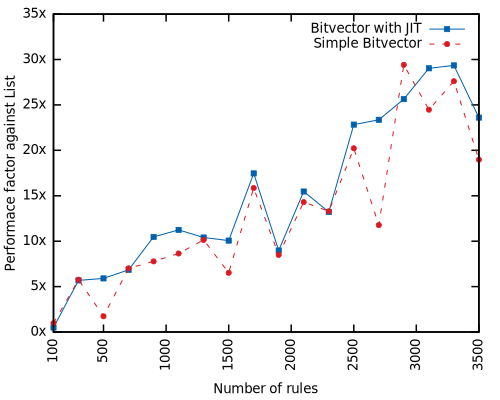
\includegraphics[height=0.9\textheight]{figures/eval_w_relative}
\end{frame}

\begin{frame}
  Time to update rule set:
  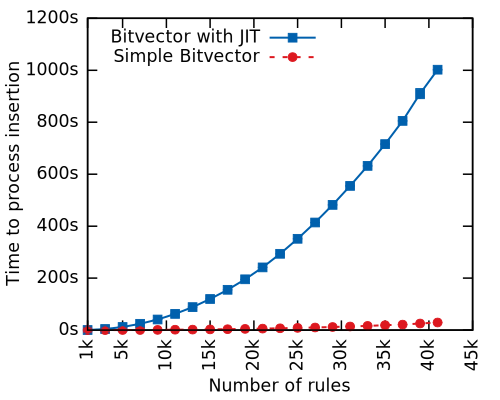
\includegraphics[height=0.9\textheight]{figures/eval_time}
\end{frame}

\begin{frame}
  Comparison of memory consumption:
  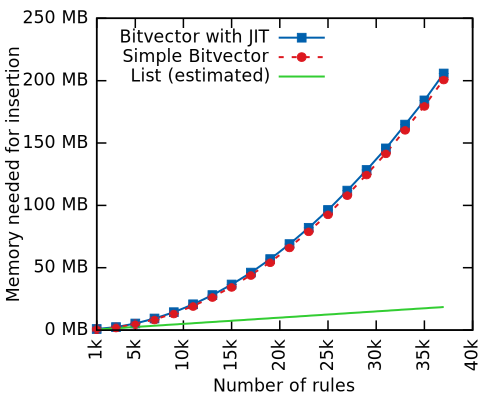
\includegraphics[height=0.9\textheight]{figures/eval_mem}
\end{frame}

\section{\scshape Conclusion}
\subsection{\scshape Results}
\begin{frame}
  \begin{tcolorbox}[colback=teal!5!white,colframe=teal!75!black,title=Important Results,drop fuzzy shadow]
    \begin{itemize}
      \item Improving the performance of the switch by using the Bitvector algorithm.
      \item Implementation of a code generator for static rule sets.
      \item Evaluation and verification of the new components.
    \end{itemize}
  \end{tcolorbox}
  \pause
  \begin{tcolorbox}[colback=blue!5!white,colframe=blue!75!black,title=Future Work,drop fuzzy shadow]
    \begin{itemize}
      \item Incremental update of the JIT funktion when the rule set changes.
      \item Optimization of the JIT funktion using traffic patterns.
    \end{itemize}
  \end{tcolorbox}
\end{frame}

\section{}
\begin{frame}
  \frametitle{\scshape Questions?}
  \centering\Huge{?}
\end{frame}

\appendix
\section{\scshape Further Results}
\begin{frame}[noframenumbering]
  \frametitle{Generating Test Rule Sets}
  \centering\includegraphics[height=0.9\textheight]{figures/rule-thirds}
\end{frame}

\begin{frame}[noframenumbering]
  Results for upper third:
  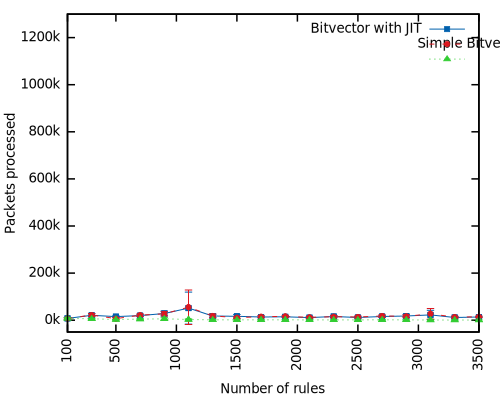
\includegraphics[height=0.9\textheight]{figures/eval_b}
\end{frame}

\begin{frame}[noframenumbering]
  Results for second third:
  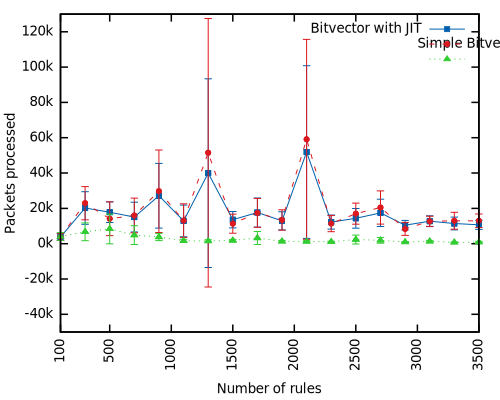
\includegraphics[height=0.9\textheight]{figures/eval_a}
\end{frame}

\begin{frame}[noframenumbering]
  Results for last third:
  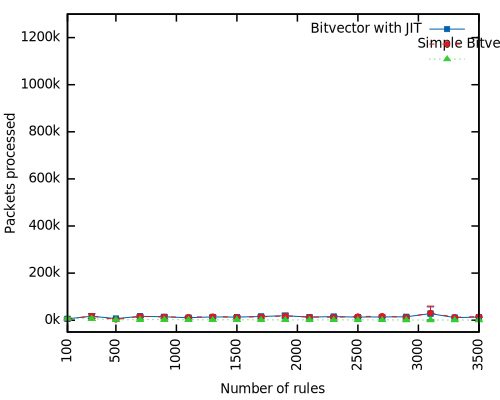
\includegraphics[height=0.9\textheight]{figures/eval_w}
\end{frame}

\begin{frame}[noframenumbering]
  Relative improvement (upper third):
  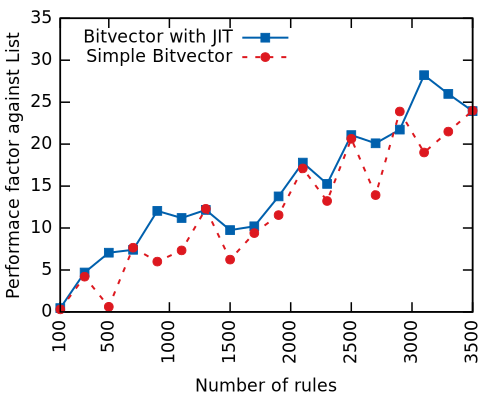
\includegraphics[height=0.9\textheight]{figures/eval_b_relative}
\end{frame}

\begin{frame}[noframenumbering]
  Relative improvement (second third):
  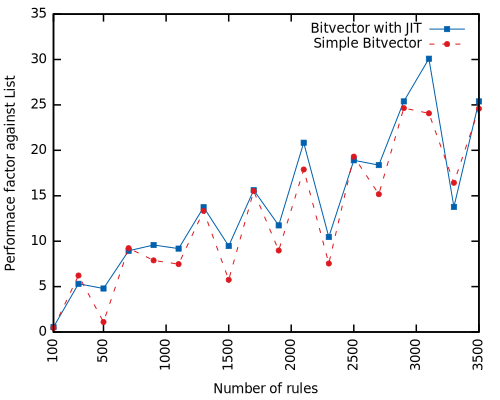
\includegraphics[height=0.9\textheight]{figures/eval_a_relative}
\end{frame}

\begin{frame}[noframenumbering]
  Relative improvement (last third):
  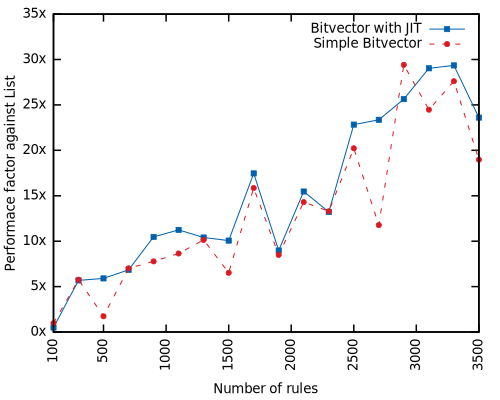
\includegraphics[height=0.9\textheight]{figures/eval_w_relative}
\end{frame}

\subsection{\scshape Generated Code}
\begin{frame}[noframenumbering]
  \only<2-7>{\begin{transparent}{0.4}}
  \only<-7>{\begin{multicols}{3}
  \lstinputlisting[
      language={[x86masm]Assembler},
      breaklines=true,
      numbers=left,
      texcl=true,
      xleftmargin=5.0ex,
      basicstyle=\tiny\ttfamily,
      keywordstyle=\bfseries\color{red},
      commentstyle=\itshape\color{grey},
      identifierstyle=\color{blue},
      morekeywords={retq,cmpq},
      numberstyle=\tiny
      ]
      {jit_listing.asm}
  \end{multicols}}
  
  \only<2-7>{\end{transparent}}

  \only<2>{\begin{textblock*}{64mm}(32mm,0.15\textheight)
    \begin{tcolorbox}[colback=red!5!white,colframe=red!75!black,title=Input into the function: 14,drop fuzzy shadow]
    \lstinputlisting[
      language={[x86masm]Assembler},
      breaklines=true,
      numbers=left,
      texcl=true,
      xleftmargin=5.0ex,
      basicstyle=\normalsize\ttfamily,
      keywordstyle=\bfseries\color{red},
      commentstyle=\itshape\color{grey},
      identifierstyle=\color{blue},
      morekeywords={retq,cmpq},
      numberstyle=\small,
      linerange={2-5},
      firstnumber=2
      ]
      {jit_listing.asm}
      \tcblower
      \centering{\includegraphics[height=0.35\textheight]{figures/match_in_tree-L1_9}}
    \end{tcolorbox}
  \end{textblock*}}
  
  \only<3>{\begin{textblock*}{64mm}(32mm,0.15\textheight)
    \begin{tcolorbox}[colback=red!5!white,colframe=red!75!black,title=Root node: compare with 5,drop fuzzy shadow]
    \lstinputlisting[
      language={[x86masm]Assembler},
      breaklines=true,
      numbers=left,
      texcl=true,
      xleftmargin=5.0ex,
      basicstyle=\normalsize\ttfamily,
      keywordstyle=\bfseries\color{red},
      commentstyle=\itshape\color{grey},
      identifierstyle=\color{blue},
      morekeywords={retq,cmpq},
      numberstyle=\small,
      linerange={7-10},
      firstnumber=7
      ]
      {jit_listing.asm}
      \tcblower
      \centering{\includegraphics[height=0.35\textheight]{figures/match_in_tree-L1_6_9}}
    \end{tcolorbox}
  \end{textblock*}}
  
  \only<4>{\begin{textblock*}{64mm}(32mm,0.15\textheight)
    \begin{tcolorbox}[colback=red!5!white,colframe=red!75!black,title=Root node: compare with 8,drop fuzzy shadow]
    \lstinputlisting[
      language={[x86masm]Assembler},
      breaklines=true,
      numbers=left,
      texcl=true,
      xleftmargin=5.0ex,
      basicstyle=\normalsize\ttfamily,
      keywordstyle=\bfseries\color{red},
      commentstyle=\itshape\color{grey},
      identifierstyle=\color{blue},
      morekeywords={retq,cmpq},
      numberstyle=\small,
      linerange={11-14},
      firstnumber=11
      ]
      {jit_listing.asm}
      \tcblower
      \centering{\includegraphics[height=0.35\textheight]{figures/match_in_tree-L1_6_9}}
    \end{tcolorbox}
  \end{textblock*}}
  
  \only<5>{\begin{textblock*}{64mm}(32mm,0.15\textheight)
    \begin{tcolorbox}[colback=red!5!white,colframe=red!75!black,title=Node C: compare with 11,drop fuzzy shadow]
    \lstinputlisting[
      language={[x86masm]Assembler},
      breaklines=true,
      numbers=left,
      texcl=true,
      xleftmargin=5.0ex,
      basicstyle=\normalsize\ttfamily,
      keywordstyle=\bfseries\color{red},
      commentstyle=\itshape\color{grey},
      identifierstyle=\color{blue},
      morekeywords={retq,cmpq},
      numberstyle=\small,
      linerange={46-49},
      firstnumber=46
      ]
      {jit_listing.asm}
      \tcblower
      \centering{\includegraphics[height=0.35\textheight]{figures/match_in_tree-L1_9_11}}
    \end{tcolorbox}
  \end{textblock*}}
  

  \only<6>{\begin{textblock*}{64mm}(32mm,0.15\textheight)
    \begin{tcolorbox}[colback=red!5!white,colframe=red!75!black,title=Node F: compare with 13,drop fuzzy shadow]
    \lstinputlisting[
      language={[x86masm]Assembler},
      breaklines=true,
      numbers=left,
      texcl=true,
      xleftmargin=5.0ex,
      basicstyle=\normalsize\ttfamily,
      keywordstyle=\bfseries\color{red},
      commentstyle=\itshape\color{grey},
      identifierstyle=\color{blue},
      morekeywords={retq,cmpq},
      numberstyle=\small,
      linerange={52-54},
      firstnumber=52
      ]
      {jit_listing.asm}
      \tcblower
      \centering{\includegraphics[height=0.35\textheight]{figures/match_in_tree-L1_9_10}}
    \end{tcolorbox}
  \end{textblock*}}
  
  \only<7>{\begin{textblock*}{64mm}(32mm,0.15\textheight)
    \begin{tcolorbox}[colback=red!5!white,colframe=red!75!black,title=Result: index 5,drop fuzzy shadow]
    \lstinputlisting[
      language={[x86masm]Assembler},
      breaklines=true,
      numbers=left,
      texcl=true,
      xleftmargin=5.0ex,
      basicstyle=\normalsize\ttfamily,
      keywordstyle=\bfseries\color{red},
      commentstyle=\itshape\color{grey},
      identifierstyle=\color{blue},
      morekeywords={retq,cmpq},
      numberstyle=\small,
      linerange={77-80},
      firstnumber=77
      ]
      {jit_listing.asm}
      \tcblower
      \centering{\includegraphics[height=0.35\textheight]{figures/match_in_tree-L1_8_9}}
    \end{tcolorbox}
  \end{textblock*}}
  
  \only<8>{
  \begin{multicols}{3}
  \lstinputlisting[
      language={[x86masm]Assembler},
      breaklines=true,
      numbers=left,
      texcl=true,
      xleftmargin=5.0ex,
      basicstyle=\tiny\ttfamily,
      keywordstyle=\bfseries\color{red},
      commentstyle=\itshape\color{grey},
      identifierstyle=\color{blue},
      morekeywords={retq,cmpq},
      numberstyle=\tiny
      ]
      {jit_listing.asm}
  \end{multicols}}
\end{frame}

\end{document}
